\documentclass{beamer}
 
\usepackage[utf8]{inputenc}
 \usetheme{Boadilla}
\usepackage{graphicx}
\usepackage{rotating}
\usepackage{ragged2e}
\title{Dynamic Models for Cash Management}
 
%Information to be included in the title page:
\subtitle{the $2^{nd} $ year review}

\author{Zimian Zhang}


\institute{Lancaster University}

\date{\today}
 
 
 
\begin{document}
\renewcommand{\raggedright}{\leftskip=0pt \rightskip=0pt plus 0cm}
 
\frame{\titlepage}
%table page
\begin{frame}
\frametitle{Outline}
\label{contents}
\tableofcontents
\end{frame}
%!!!!!!!!!!!!!
 
%the FIRST page
\section{Introduction}
\begin{frame}
\frametitle{Introduction}

\begin{itemize}
\item \hyperlink{cashproblem}{What is ``cash management problem''?}
\pause
\item Models from literature
\pause
\item Wrap-up from the $1^{st}$ year's work

\end{itemize}
\end{frame}
%!!!!!!!!!!!!!
\begin{frame}
\label{cashproblem}
\frametitle{\hyperlink{intro}{What is cash management problem?}}

\begin{columns}
\column{0.4\textwidth}
\begin{itemize}
\item<3->With insufficient cash holding level, a company might expose to the risk of cash deficit, which might cause a great amount of penalty.
\item<4->On the other hand, a high cash-holding level normally means the inefficient use of firm's resource, which would constrain firm's future profitability.
\end{itemize}
\column{0.6\textwidth}
\includegraphics<2->[scale = 0.27]{holdingCost.png}
\end{columns}
\end{frame}



\begin{frame}
\frametitle{Models from literature}

\begin{small}
\begin{itemize}

\item<2-> A basic cash management model 

\includegraphics<3>[scale = 0.35]{basicModel.png}
\end{itemize}

\begin{itemize}
\item<4-> A CM model in a randomly varying environment  (Hinderer, Waldmann, 2001)

\includegraphics<5>[scale = 0.25]{EnvMod.png}
\end{itemize}

\begin{itemize}
\item<6-> A CM model with two accounts (Bensoussan, Chutani, and Sethi, 2009)

\includegraphics<7>[scale = 0.25]{otherTwoAsset.png}
\end{itemize}

\begin{itemize}
\item<8-> A CM model with different cash demand (Nascimento, and Powell, 2010)

\includegraphics<9>[scale = 0.25]{mutualFund.png}
\end{itemize}


\begin{itemize}
\item<10-> A CM model with different cash sources (Sato, and Sawaki, 2009)

\includegraphics<11>[scale = 0.25]{twoSource.png}

\end{itemize}
\end{small}



\end{frame}


\begin{frame}
\frametitle{Motivation}
\begin{itemize}
\item<2->Most literature discussed cash-holding policy only.

\item<3->We study the cash holding strategy with other ``cash related activities''.

\item<4->We propose a holistic CM model in financial sector (e.g. mutual funds, commercial banks, pension funds or insurance companies)


\end{itemize}


\end{frame}


\begin{frame}
\frametitle{A holistic model in financial sector}
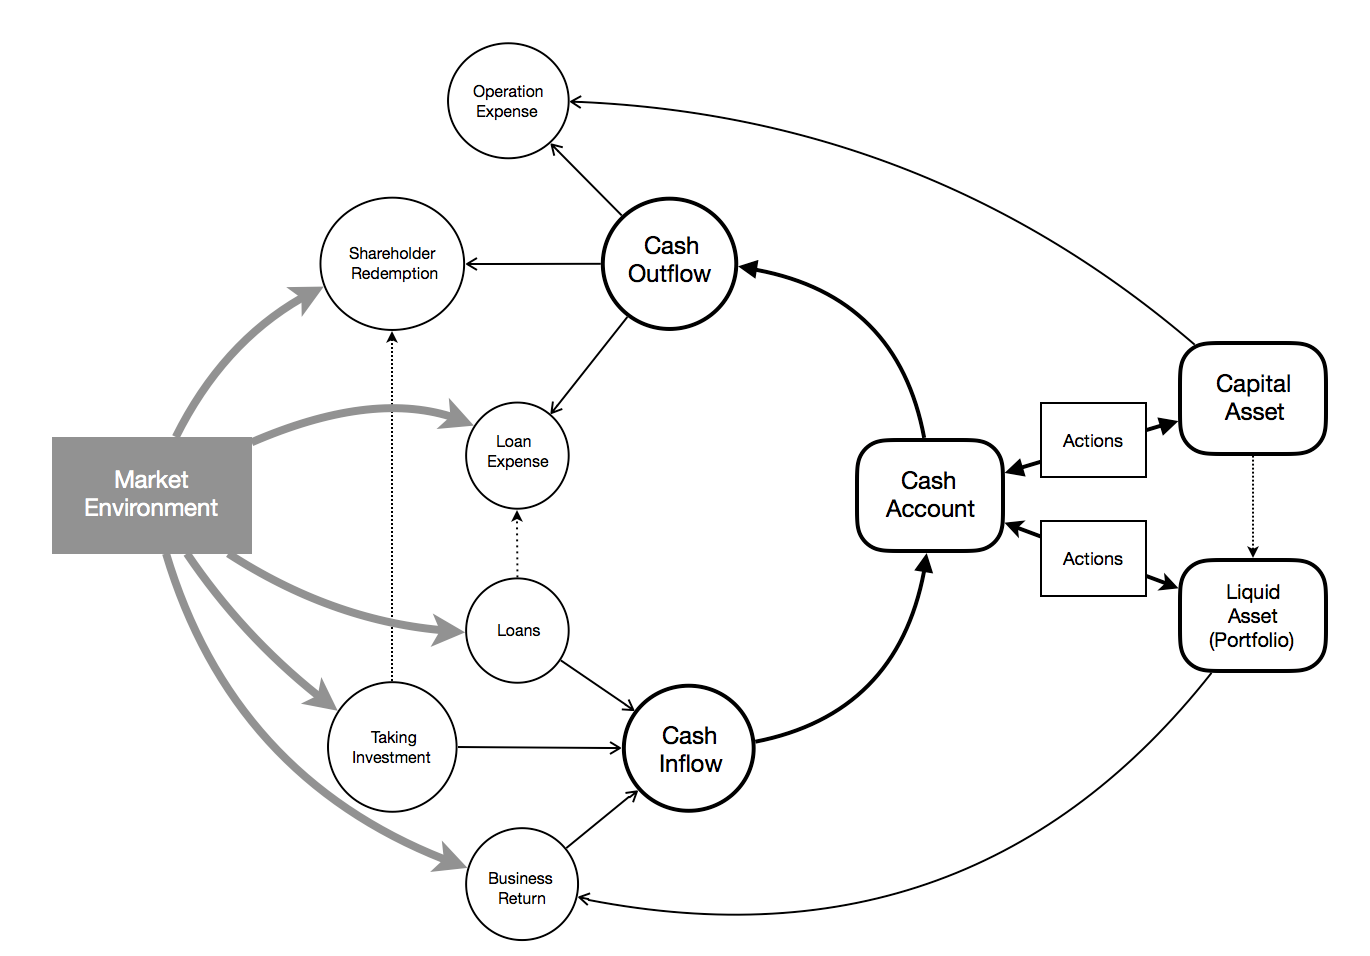
\includegraphics[scale = 0.25]{Holistic.png}

\end{frame}
\begin{frame}
\frametitle{Wrap-up from 1st year's work}


\begin{itemize}
\item<2->Model: A two-assets CM model.


\includegraphics<3>[scale = 0.25]{twoAcMod.png}

\item<4->Methodology: Dynamic Programming

\begin{itemize}
\item<5-7> Objective Function: Maximise the sum of return in every time periods.

\only<5>{\begin{block}{Objective Function}
$$\max_{a \in \prod }  \mathbb{E}\left\{ \sum_{t = 0} ^ T ry_t\right\}.$$
\end{block}}
\item <6-7>Recursion Method:

\only<7>{\begin{block}{Recursion Method:}
\begin{enumerate}
\item $$V^{T+1}_{\textbf{s}} = 0$$

\item $$V^{t}_{\textbf{s}}(\textbf{a}) = ry + \int^{\infty}_{-\infty} p_\theta V^{t+1}_{\textbf{s}'}d\theta.$$

\item $$a^* = \underbrace{\arg \max}_{a \in A_{\textbf{s}}} \left\{      ry + \int^{\infty}_{-\infty} p_\theta V^{t+1}_{\textbf{s}'}d\theta \right\}$$
\item $$V^{t}_{\textbf{s}} = \max_{a \in A_{\textbf{s}}} \left\{      ry + \int^{\infty}_{-\infty} p_\theta V^{t+1}_{\textbf{s}'}d\theta \right\}.$$
\end{enumerate}
\end{block}}
\end{itemize}
\end{itemize}
\end{frame}

\begin{frame}
\frametitle{Wrap-up from 1st year's work}
\begin{itemize}
\item Result: a solution suggested by DP method

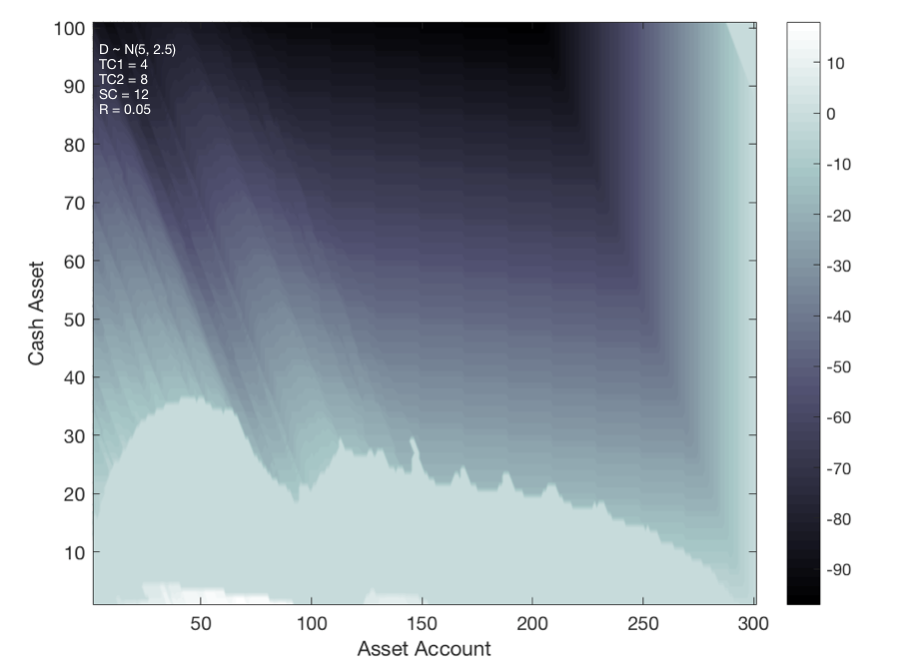
\includegraphics[scale = 0.25]{ResultFirstYear_rdy.png}


\end{itemize}
\end{frame}

\section{Overall research project}
\begin{frame}
\frametitle{Research Steps}
\begin{itemize}
\item <2-> Step I: Examine the two assets CM model

\includegraphics<3>[scale = 0.25]{twoAcMod.png}

\item <4-> Step II: Introduce the loan options into the CM model

\includegraphics<5>[scale = 0.45]{loan.png}


\item <6-> Step III: Complete the holistic CM model and propose an effective way to solve it (approximate dynamic programming).

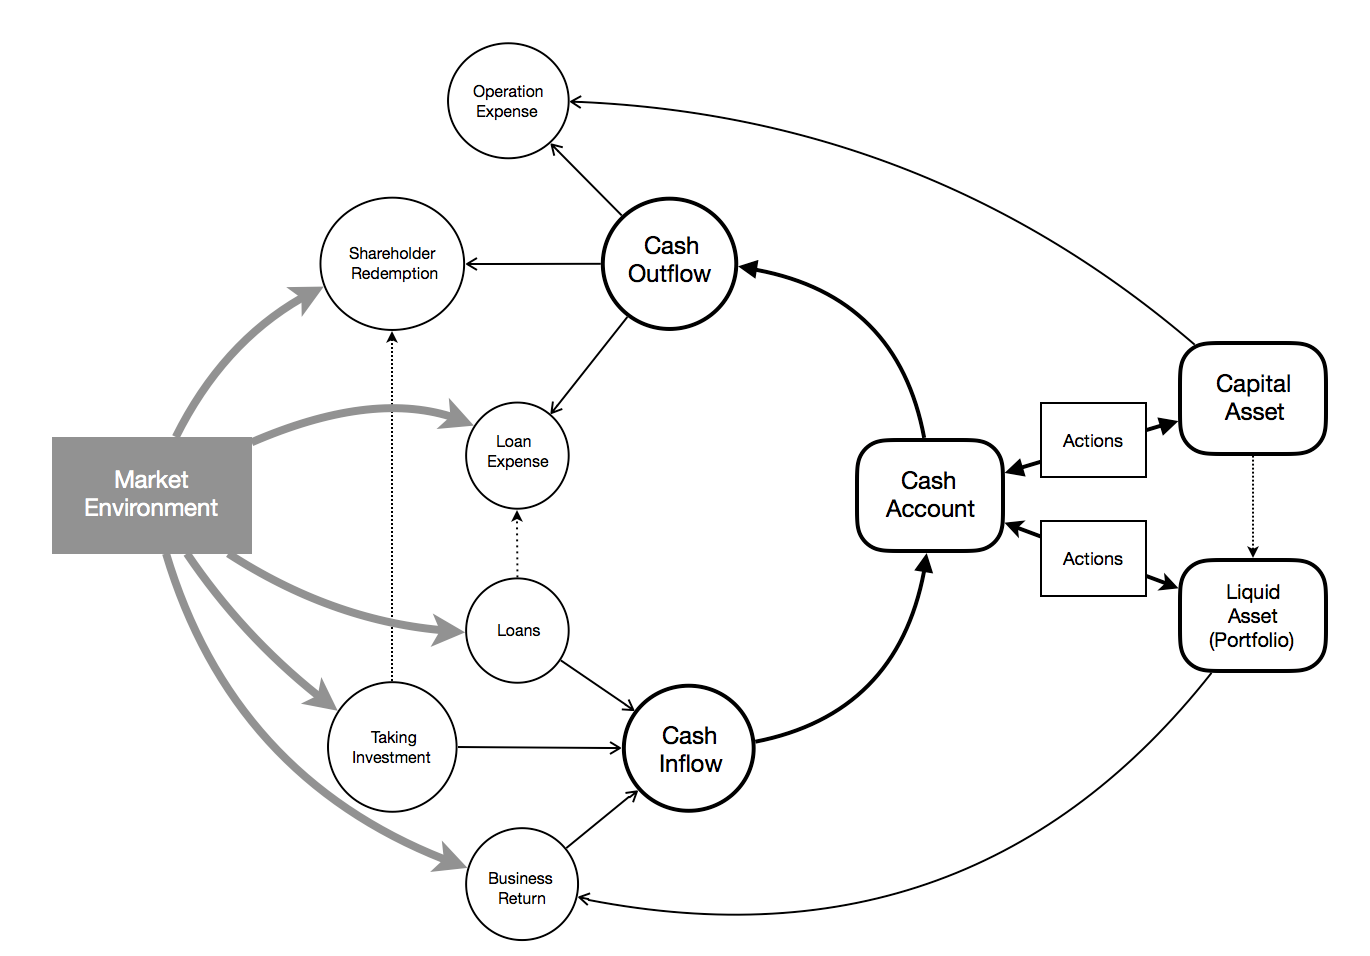
\includegraphics[scale = 0.18]{Holistic.png}


\end{itemize}
\end{frame}
\begin{frame}
\frametitle{Thesis structure}


\begin{itemize}
\item Chapter I.	Introduction
\item Chapter II. Literature Review
\begin{itemize}
\item  2.1 Literature Review of Cash Management in OR
\item  2.2 Literature Review of  Cash Flows in Financial Sector
\item 2.3 A Holistic Model based on Literature
\end{itemize}
\item Chapter III. Methodology
\begin{itemize}
\item  3.1 Introduction to Dynamic Programming
\item  3.2 Introduction to Approximate Dynamic Programming
\end{itemize}
\item Chapter IV. A Two Assets Cash Management Model
\begin{itemize}
\item  4.1 Model Summary
\item  4.2 Dynamic Programming Method
\item 4.3 Numeric Experiment
\end{itemize}
\end{itemize}
\end{frame}


\begin{frame}
\frametitle{Thesis structure}


\begin{itemize}


\item Chapter V. A Cash Management Model with Loans
\begin{itemize}
\item  5.1 Model Summary
\item  5.2 Dynamic Programming Method
\item  5.3 Heuristic Method: One Step Policy Improvement
\item  5.4 Numeric Experiment
\end{itemize}

\item Chapter VI. Approximate Dynamic Programming in Cash Management Models
\begin{itemize}
\item  6.1 Temporal Difference Method
\item  6.2 Eligibility Trace Method
\item  6.3 Function Approximation
\end{itemize}
\item Chapter VII. Conclusion
\end{itemize}

\end{frame}

\section{Current progress}
\begin{frame}
\frametitle{Current progress}
\begin{itemize}
\item Modify the two asset model and the performance of the cash holding strategy
\item Introduce the loan options into the model and using DP and heuristic method to solve the model
\item Approximate Dynamic Programming: Temporal Difference and Eligibility Trace in the CM model
\end{itemize}
\end{frame}

\begin{frame}
\frametitle{The two assets CM model}
\begin{itemize}
\item Objective function: Maximising net profits $$\max \sum^\infty _{t = 0}\gamma^t  \{ rr \cdot y_t - D_t - \Gamma_t - SC_t \}.$$
\item A partially fixed and partially proportional transaction cost function$$\Gamma(a) =  (K_c + k_c a) \cdot 1_{\{ a < 0\}} + (K_a +k_aa)\cdot 1_{\{a>0\}}$$
\item Options of declaring bankruptcy

\end{itemize}
\end{frame}



\begin{frame}
\frametitle{An optimal solution of the modified model}
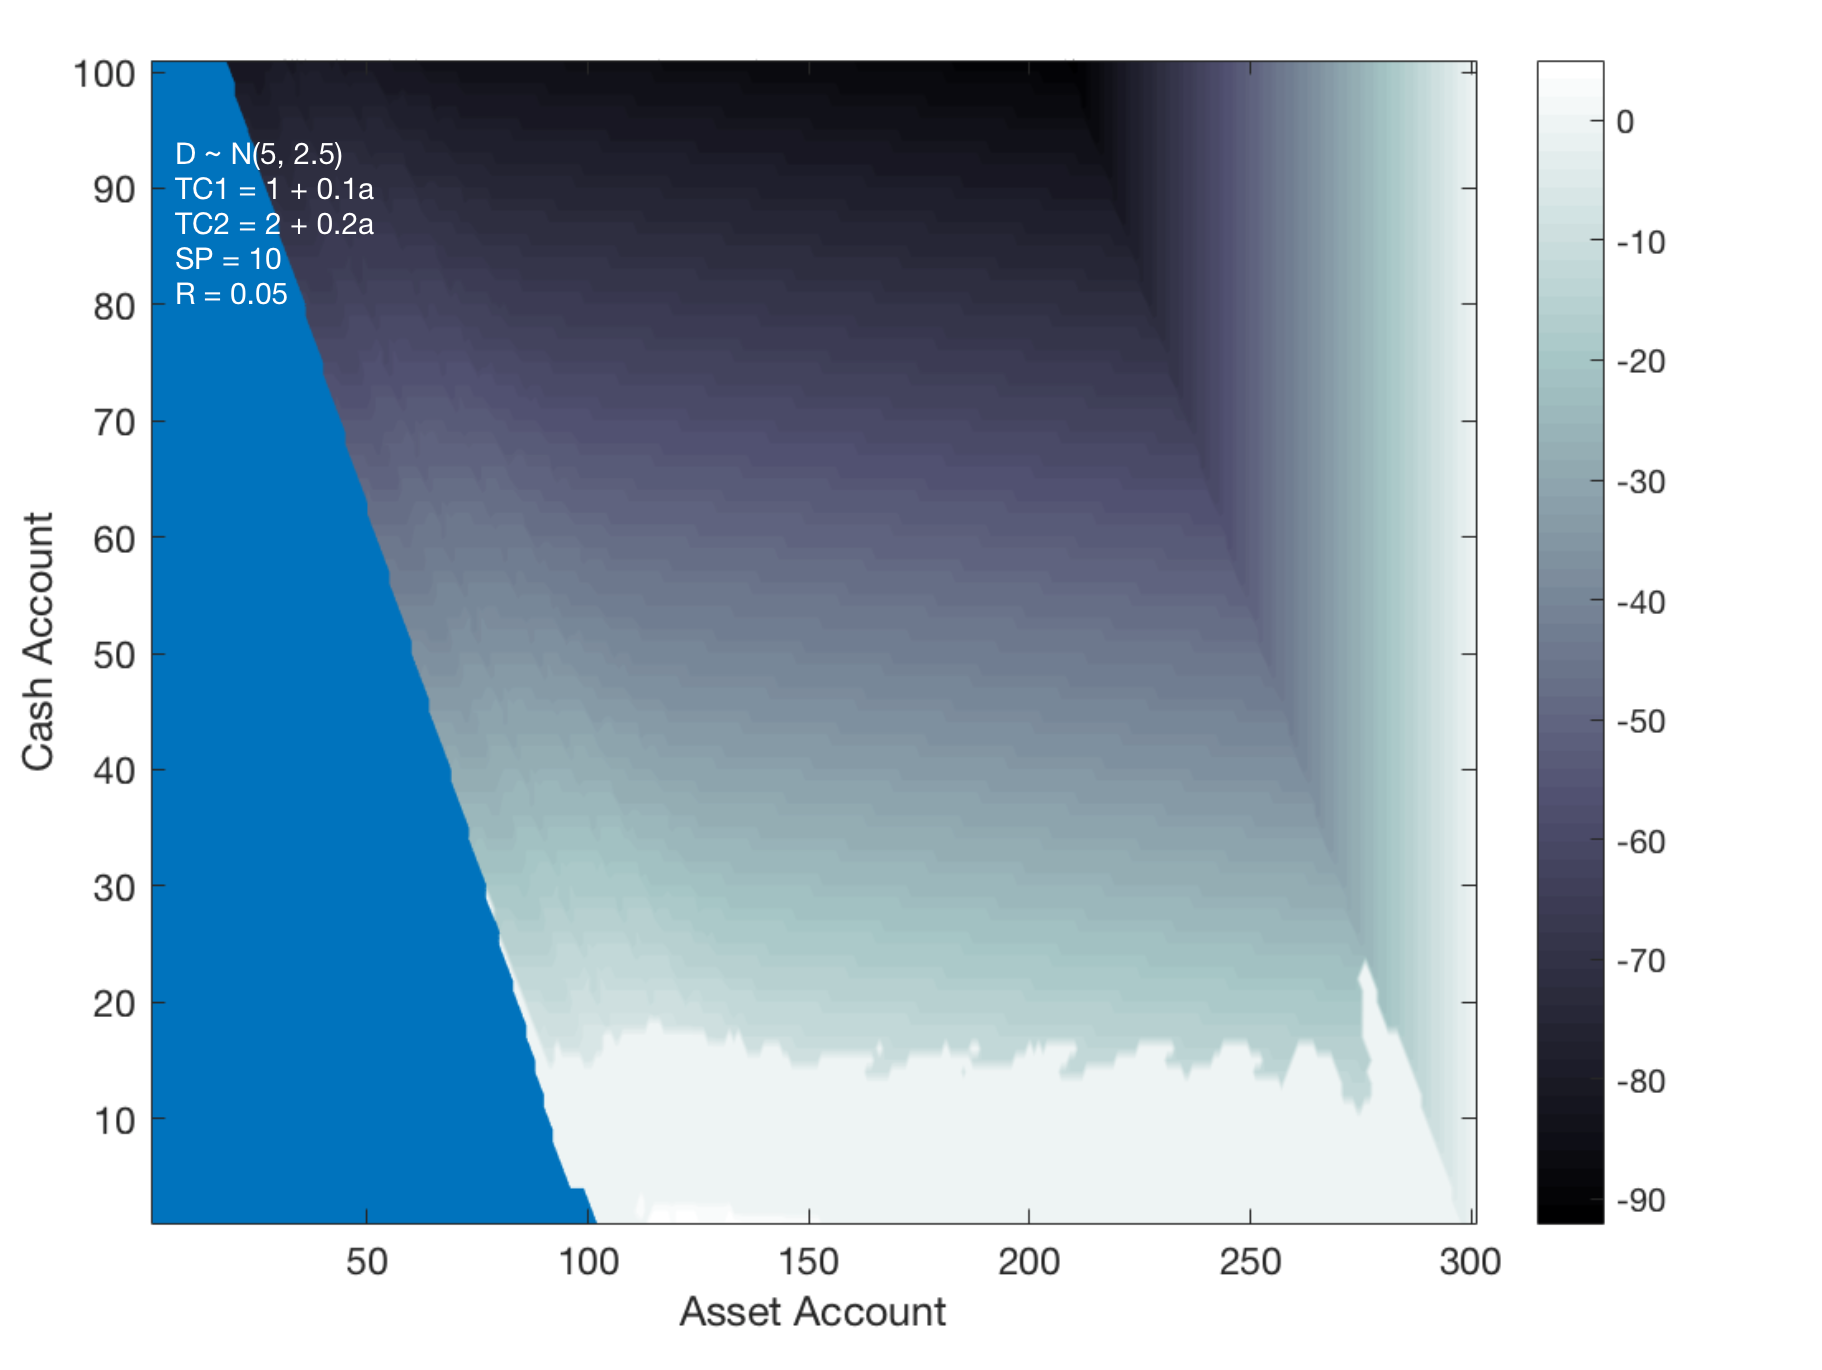
\includegraphics[scale = 0.25]{ModifiedModel.png}
\end{frame}

\begin{frame}
\frametitle{Simulation of the strategy}
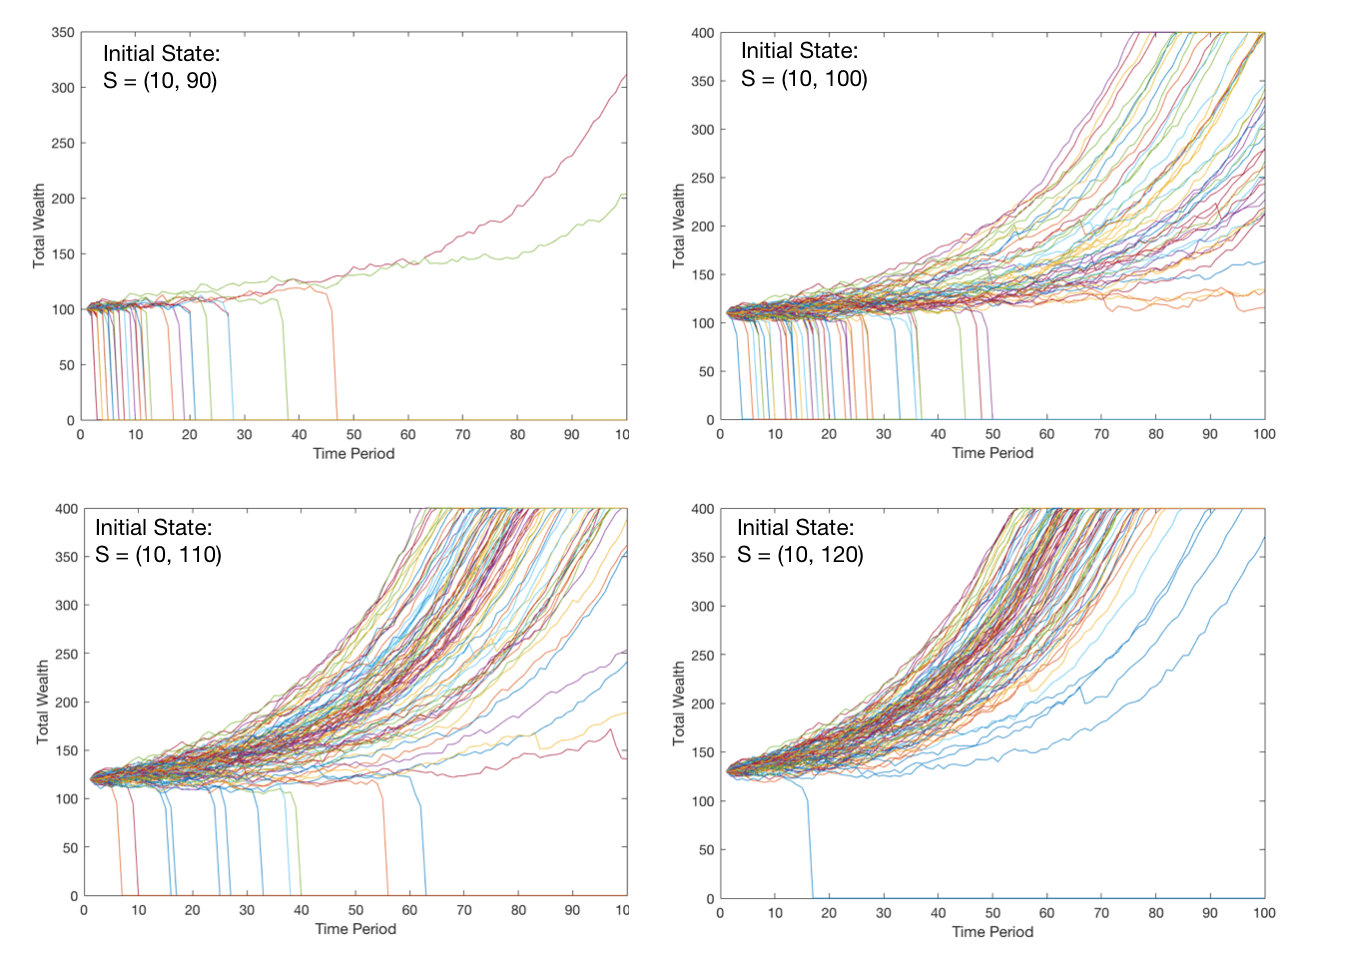
\includegraphics[scale = 0.4]{simu.png}
\end{frame}

\begin{frame}
\frametitle{Probability of going bankrupt}
\begin{itemize}
\item At stage 0 (the last period of time planning horizon), any state $S_{x, y}$ with $y \neq 0$ has value (probability of going bankrupt) equal to 0 and any state $S_{x, y}$ with $y = 0$ has value (probability of going bankrupt) equal to1.
\item for any stage $k: k \geq 1$

\[
\begin{split}
V_{[x,y]}^{k} =& \sum P\left\{\left.S_{(0,0)}:W(S_{x,y}) = S_{(0,0)}\right|a = A^*(S_{x,y})\right\} 
\\ 
+ & \sum P\left\{ \left. S_{x',y'}:W(S_{x,y}) = S_{x',y'} \right| a = A^* (S_{x,y})\right\}  V_{[x',y']}^{k-1}
\end{split}
\]
where $V_{[x,y]}^{k} $ is the probability that the company will eventually going bankrupt if it is in state $S_{x,y}$ at stage $k$
\end{itemize}
\end{frame}

\begin{frame}
\frametitle{Probabilities of going bankrupt in each state: Simulation result and Backward calculation result}
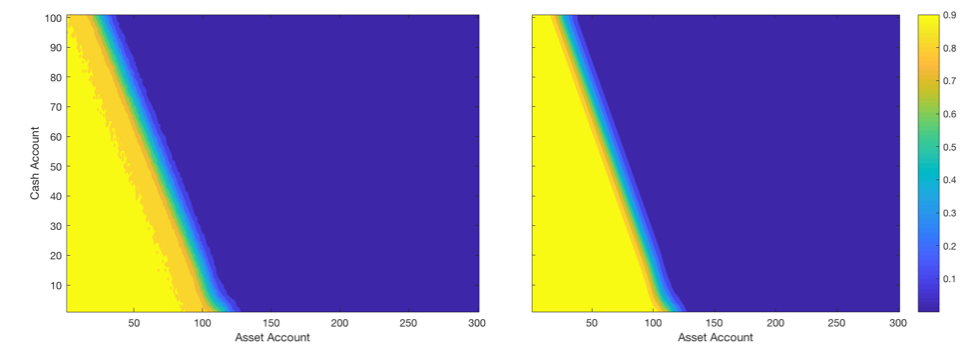
\includegraphics[scale = 0.35]{prob.png}
\end{frame}

\begin{frame}
\frametitle{Cash management with loan options}
In reality, once company's income could not cover its cash demand, instead of selling asset and jeopardising future profitabilities, managers tend to take loans from other companies or financial intermediaries.



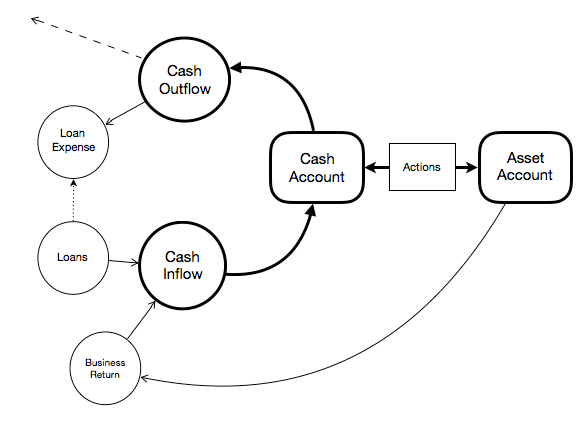
\includegraphics[scale = 0.4]{loan.png}


\end{frame}

\begin{frame}
\frametitle{Cash management with loan options}
\begin{itemize}
\item State: $S_{x,y,z}$ where $x$ and $y$ represent the current cash and asset level and $z$ represent the remaining times of loan repayment.
\item Loan Repayment $LP$: let $L$ be the loan size, $lr$ be the loan rate and once the manager take the loan, he has to make an equally amount of repayment in following $N$ time periods. Then for each time period, he has to pay $$LP = L \cdot \frac{lr \cdot (1+lr)^N}{(1+lr)^N-1}$$
\item We assume that companies with debt unpaid cannot take more loans.
\item At time $t$, if the manager take the loan, then the cash inflow increases by $L$ amount and its loan state $s$ changes from $0$ to $N$. In the following $N$ time periods, the company's cash demand will increase by LP amount and $z$ value decreases by $1$. 
\end{itemize}
\end{frame}

\begin{frame}
\frametitle{Cash management with loan options}
\begin{itemize}
\item<2-> Limitation: we can formulate this model as a Markov Decision Process problem. But the computation cost will increase dramatically.
\item<3->  Heuristic Method: One-step policy improvement.


\includegraphics<4->[scale=.2]{oneImprov}

\end{itemize}
\end{frame}

\begin{frame}
\frametitle{Simulation results of one-step policy improvement}
Assume there is only one loan available on the market: $L = 40, lr = 0.03, N = 40$


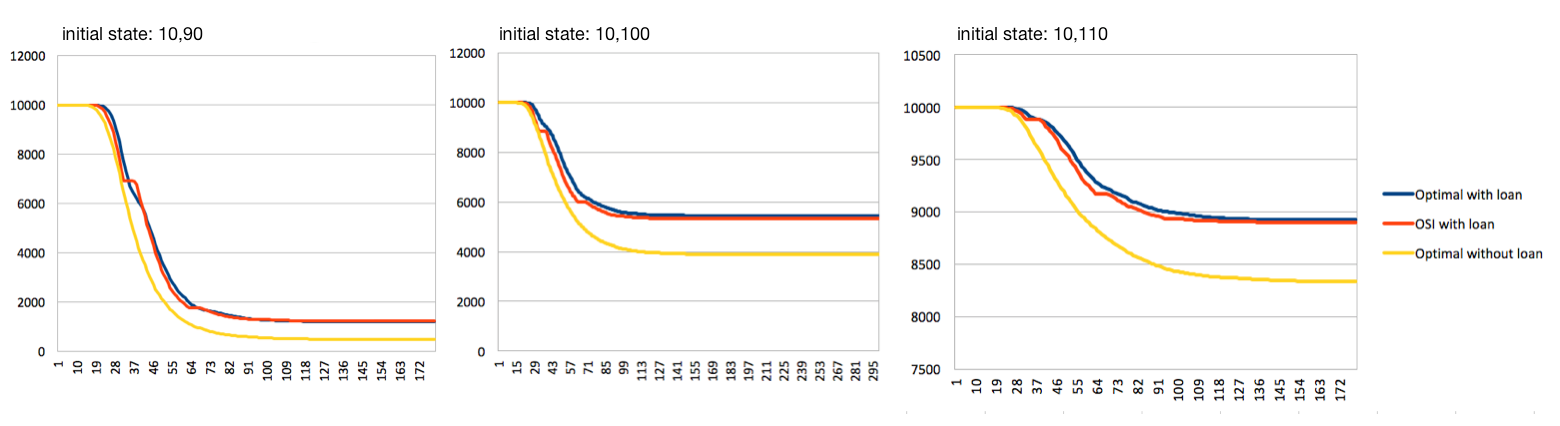
\includegraphics[scale=.22]{oneStep}
\end{frame}

\begin{frame}
\frametitle{The cost of dynamic programming}
Updating rule:
\begin{small}
$$ a(S_{x,y}) = \arg\max \left\{   
R_t^{a}(S_{x,y}) + \gamma \sum_{S_{x',y'}\in S} V^{a}_{t-1}(S_{x',y'})
\mathbb{P}\left\{S_{x',y'}:W(S_{x, y}) = S_{x', y'} \right\}
 \right\} $$
$$V^a(S_{x,y}) =  R_t^{a}(S_{x,y}) + \gamma \sum_{S_{x',y'}\in S} V^{a}_{t+1}(S_{x',y'})
\mathbb{P}\left\{S_{x',y'}:W(S_{x, y}) = S_{x', y'} \right\}.$$
\end{small}
\includegraphics<2->[scale=.16]{dp}

\end{frame}

\begin{frame}
\frametitle{One-step Temporal Difference}
Updating rule: $V(S_{x,y}|A=a^\pi(S_{x,y})) :=$
\begin{small}
 $$V(S_{x,y}|A=a^\pi(S_{x,y})) + \alpha \left[ R + \gamma V(S_{x',y'}|A=a^\pi (S_{x',y'}))\right] - V(S_{x,y}|A=a^\pi(S_{x,y}))$$ 
 \end{small}
 where $\alpha$ is the update step size parameter.

\includegraphics<2->[scale=.4]{OneTD}
\end{frame}

\begin{frame}
\frametitle{n-step Temporal Difference}
\includegraphics[scale=.4]{nstep}
\end{frame}
\begin{frame}
\frametitle{Result of 1 step TD}
\begin{itemize}
\item Limitation of TD method: Speed of convergence.

\includegraphics<2>[scale=.34]{1TD}

\item<3-> How to improve?
\begin{itemize}
\item change the step size parameter $\alpha$
\item use eligibility trace method 
\item use function approximation

\end{itemize}

\end{itemize}
\end{frame}

\section{Research plans for next year}
\begin{frame}
\frametitle{Research Plan for next year}
\begin{itemize}
\item Study temporal difference and eligibility trace method and apply it into cash management models
\item Study approximate functions in ADP; Find a function that can approximate values in DP model.
\item Develop the literature review in terms of cash flows in financial companies and modify the holistic model.
\item Do numeric experiments for each cash management model and finish the thesis.
\end{itemize}
\end{frame}

\begin{frame}
\frametitle{Time table for next year}

\begin{table}

\centering
\begin{tabular}{| l | l |}
\hline
\hline
September & Use ET in two assets model;\\
\hline
October & Numeric experiment of two assets model;\\
& Study the function approximate in ADP;\\
\hline
November & Continue in the study of the function approximate in ADP;\\

& Write the fourth chapter of the thesis;\\
\hline
December & Finish the fourth chapter of the thesis;\\
& Continue in the study of the function approximate in ADP;\\
\hline
January & Use TD and ET in the CM model with loans;\\
& Write the fifth chapter of the thesis;\\
\hline
Feburary & Use Approximate Functions in the CM model with loans;\\
& Write the fifth chapter of the thesis;\\
\hline
March & Numeric experiment of the CM model with loans\\
& Finish the fifth chapter of the thesis;\\
\hline
\end{tabular}
\end{table}
\end{frame}




\begin{frame}
\frametitle{Time table for next year}
\begin{table}

\centering
\begin{tabular}{| l | l |}
\hline

\hline
April & Read more literature about cash flows in financial sector\\
& Modify the holistic model\\
\hline
May & Read more literature about cash flows in financial sector;\\
& Use TD and ET in the holistic model\\
\hline
June & Write up the sixth chapter of the thesis\\
& Use approximate functions in the holistic model\\
\hline
July & Write up the sixth chapter of the thesis\\
& Numeric experiment in the holistic model\\
\hline
August & Finish the sixth chapter of the thesis;\\
& Write the literature review of the thesis;\\
\hline
September & Write the methodology of the thesis;\\
& Finish the first draft of the thesis;\\

\hline
\hline
\end{tabular}
\end{table}

\end{frame}

\begin{frame}

\includegraphics[scale=.4]{tky}
\end{frame}

\end{document}